\problemname{Svampar}
\noindent

\illustration{0.30}{mycelial_network.jpg}{}{}

För att kunna driva din nya AI-startup behöver du kunna utföra parallella beräkningar på stor skala.
En stark kandidat för detta visar sig vara svampar!
För att beräkna saker har du ett kluster av $N$ stycken svampar numrerade från $1$ till $N$.
Du vill nu ladda in vikterna för ett neuralt nätverk i svamparna.
Varje svamp förvarar ett tal, som till början är $0$.

För att ändra på svamparnas tal kan du utföra en \textit{runda}.
För varje runda anger du en instruktion till varje svamp.
Alla dessa instruktioner utförs sedan samtidigt.
Låt $P[i]$ beteckna värdet på svamp $i$ innan rundan och $A[i]$ värdet på svamp $i$ efter rundan.
De tillgängliga operationerna för svamp $i$ är då:
\begin{alignat*}{3}
\texttt{\makebox[2em][l]{p\ \ :}}             & A[i] & = & P[i] & & \quad \text{behåll värdet från innan.} \\
\texttt{\makebox[2em][l]{< j:}}           & A[i] & = & P[j]\ \texttt{<<}\ 1 & & \quad \text{där \texttt{<<} betecknar bitvis  vänsterskift.} \\
\texttt{\makebox[2em][l]{> j:}}           & A[i] & = & P[j]\ \texttt{>>}\ 1 & & \quad \text{där \texttt{>>} betecknar bitvis högerskift.} \\
\texttt{\makebox[2em][l]{+ j:}}           & A[i] & = & P[j] + 1 & & \quad \text{där \texttt{+} betecknar addition.} \\
\texttt{\makebox[2em][l]{\textasciicircum\ j:}} & A[i] & = & P[i]\ \texttt{\textasciicircum}\ P[j] & & \quad \text{där \texttt{\textasciicircum} betecknar bitvis XOR.} \\
\texttt{\makebox[2em][l]{\& j:}}          & A[i] & = & P[i]\ \&\ P[j] & & \quad \text{där \texttt{\&} betecknar bitvis AND.} \\
\texttt{\makebox[2em][l]{| j:}}           & A[i] & = & P[i]\ |\ P[j] & & \quad \text{där \texttt{|} betecknar bitvis OR.} 
\end{alignat*}


Se till att läsa beskrivningen av operationerna noggrant. Du kan hitta en definition av alla bitvisa operationer här
\footnote{\href{https://en.wikipedia.org/wiki/Bitwise\_operations\_in\_C\#Bitwise\_operators}{https://en.wikipedia.org/wiki/Bitwise\_operations\_in\_C\#Bitwise\_operators}}.
Svamparna kan förvara godtyckligt stora tal. 

Du får nu $N$ vikter $w_1, w_2, \dots, w_N$ och behöver hitta en sekvens rundor som får $A[i]=w_i$ för alla $i$.

Ju färre rundor du använder, desto mer poäng får du. I testdatan är $N$ alltid $512$.

\section*{Indata}
Den första raden av indata innehåller heltalet $N$ ($N=512$), antalet svampar.
Anledningen att detta är en del av indata är för att underlätta testning av din lösning på mindre $N$.

Den andra raden innehåller heltalen $w_1, w_2, \dots, w_N$ ($0 \leq w_i \leq 255$),
vikterna i det neurala nätverket.

\section*{Utdata}
Skriv först ut heltalet $r$, antalet rundor din lösning använder.

Skriv därefter ut $r$ rader, där varje rad beskriver en runda.
För varje runda, skriv ut varje operation som ska utföras, vänster till höger.
En operation skrivs ut på samma format som i beskrivningen ovan.
För varje operation krävs det att $1 \leq j \leq N$.

\section*{Poängsättning}
Din lösning kommer att testas på ett antal testfall.
Om den någonsin skriver ut en sekvens rundor som är ogiltig eller som inte producerar rätt vikter får du noll poäng.

Annars, låt $R_{max}$ beteckna det största antalet rundor du använder över alla testfall.
Då får du poäng enligt följande styckvis linjär funktion.

\begin{figure}[h]
  \centering
  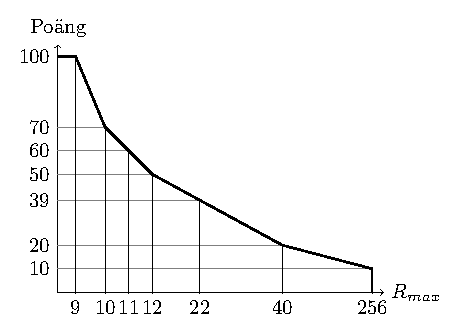
\includegraphics[width=0.4\textwidth]{scoring-se.pdf}

  \parbox{0.4\textwidth}{\centering
    Antalet poäng du får för en given $R_{max}$.\\
    Notera att x-axeln inte är linjär.
  }
\end{figure}

Om $R_{max} \leq 9$ så får du 100 poäng.
Poängvärdet för $9 \leq R_{max} \leq 20$ anges även i nedanstående tabell.

\begin{center}
  \noindent
  \begin{tabular}{| l | l |}
    \hline
    $R_{max}$ & Poäng \\ \hline
    $9$            & $100$ \\ \hline
    $10$           & $70$ \\ \hline
    $11$           & $60$ \\ \hline
    $12$           & $50$ \\ \hline
    $13$           & $48$ \\ \hline
    $14$           & $47$ \\ \hline
    $15$           & $46$ \\ \hline
    $16$           & $45$ \\ \hline
    $17$           & $44$ \\ \hline
    $18$           & $43$ \\ \hline
    $19$           & $42$ \\ \hline
    $20$           & $41$ \\ \hline
  \end{tabular}
\end{center}
